\section{Introduction}

This is the user manual for the Vitensenteret mobile app developed in 2016. The mobile application consists of a series of minigames, each of which have corresponding room or element in Vitensenteret's exhibition. It's meant to be played like an exploring game, where bluetooth beacons notify the player when he/she finds a game in the exhibition, but can also be played without the beacons.
\\\\
This manual will explain how the application works and how to play the different games.


\section{Requirements}
Device with Android 4.4 KitKat or newer.\\
Bluetooth Low Energy (Optional, for beacons)\\
An internet connection (Optional, for submitting robot at the end)\\


\section{Installation}
See Appendix \ref{appendix:installation_guide}, Installation Guide

\section{Get to know the application}
\subsection{First run}
When first running the application you will be asked to select your preferred language, as seen in Figure \ref{fig:choose_lang}. Simply click one of the flags and the rest of the application will be in that language.
There is also a welcome screen with a introduction to the app and game story. See fig. \ref{fig:welcome_screen}.


\begin{figure}[H]
  \begin{minipage}[t]{0.35\textwidth}
    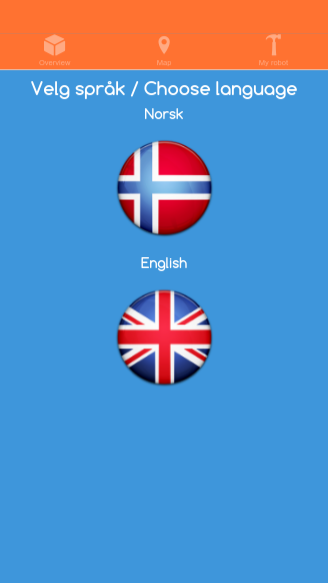
\includegraphics[width=\textwidth]{images/app/chooseLanguage.png}
    \caption{The ``choose language" app view}
    \label{fig:choose_lang}
  \end{minipage}
  \hfill
  \begin{minipage}[t]{0.35\textwidth}
    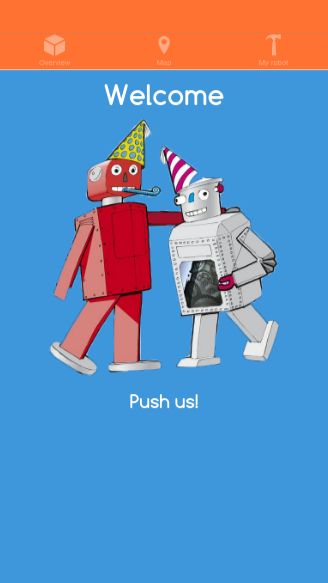
\includegraphics[width=\textwidth]{images/app/welcomeScreen.png}
    \caption{The ``Welcome screen" app view}
    \label{fig:welcome_screen}
  \end{minipage}
\end{figure}

\subsection{Game Overview}

\begin{figure}[H]
    \centering
    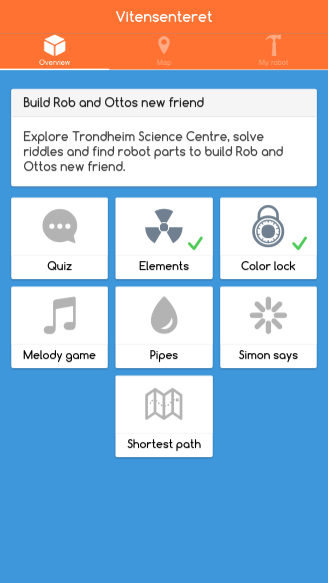
\includegraphics[width=0.5\textwidth]{images/app/overview_finished.png}
    \caption{The ``Game overview" app view, with some games finsihed.}
    \label{fig:overview_finished}
\end{figure}

The game overview, as seen in figure \ref{fig:overview_finished}, is the home screen of the application, where one can find the minigames and their status. They can be either semi-transparent, which means they have not been found yet (with beacons activated, as seen in figure \ref{fig:overview_beacons}), colored with a checkmark, which means they have been completed, or colorless, which means they have not yet been completed.\\\\
By clicking a game card a popup will be shown, telling a short story and instructing the player how to play the game. From there the player can start the game.

\begin{figure}[H]
    \centering
    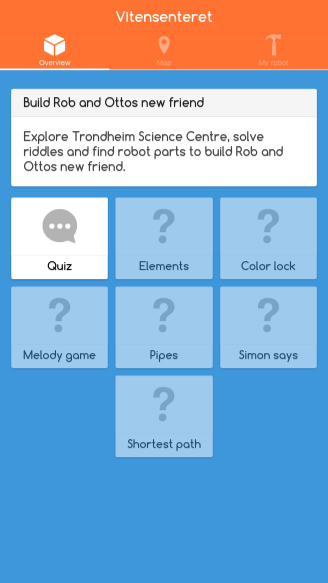
\includegraphics[width=0.5\textwidth]{images/app/overview_beacons.png}
    \caption{The ``Game overview" app view, with beacons enabled.}
    \label{fig:overview_beacons}
\end{figure}


\subsection{Tabs}
The three non-game views can be navigated to by using tabs located at the bottom or top of the screen, depending on what OS you are using. These can take you to the minigame overview, map or robot builder.

\subsection{Map}
The map shows a floor-plan of Vitensenteret's exhibition, with the minigames's locations plotted, as seen in figure \ref{fig:map}. One can zoom and pan the map.

\begin{figure}[H]
    \centering
    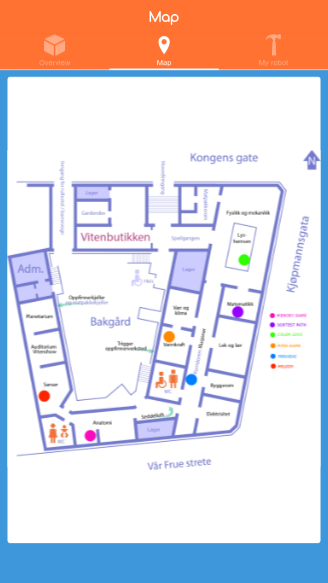
\includegraphics[width=0.5\textwidth]{images/app/Map.png}
    \caption{The ``Map" app view.}
    \label{fig:map}
\end{figure}

\subsection{Robot builder}
In the robot builder view one can see the different robot parts one has collected by winning games, as well as switch which part and color one wants for the robot, as seen in figure \ref{fig:parts}.

\begin{itemize}
    \item By clicking the robot at the top left one can zoom in on it.
    \item By clicking the arrows one can change the selected robot part.
    \item By clicking the robot part in the list a color and lightness selector is opened, where one can change the color of the robot. See figure \ref{fig:parts_colors}.
\end{itemize}



\begin{figure}[H]
    \centering
    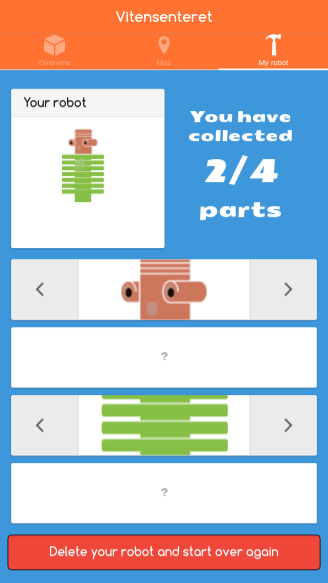
\includegraphics[width=0.5\textwidth]{images/app/parts.png}
    \caption{The ``Robot parts" app view.}
    \label{fig:parts}
\end{figure}


\begin{figure}[H]
    \centering
    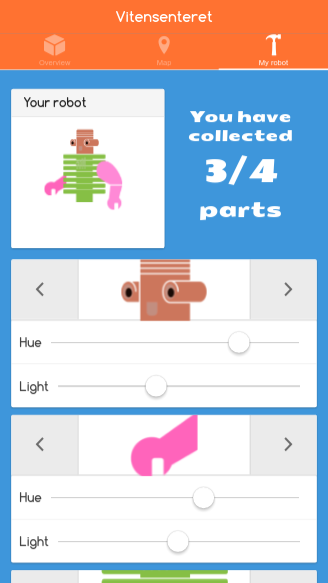
\includegraphics[width=0.5\textwidth]{images/app/parts_colors.png}
    \caption{The ``Robot parts" app view, with the color customization sliders open.}
    \label{fig:parts_colors}
\end{figure}



\section{Games}

\begin{figure}[H]
    \centering
    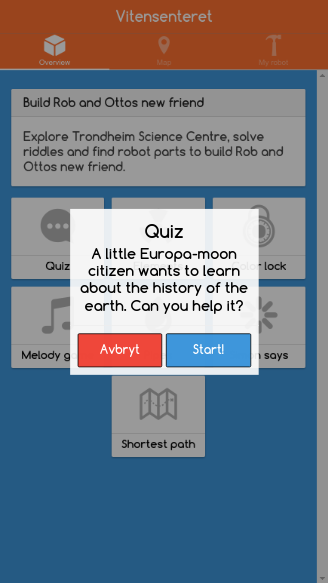
\includegraphics[width=0.5\textwidth]{images/app/overview_start_game.png}
    \caption{An example of the game story.}
    \label{fig:overview_start_game}
\end{figure}

The minigames have a common story where the player is helping two robots find robot parts for a new robot. They don't need to be done in a certain order, but as there are only four types of robot parts, and seven minigames, one will win all the robot part types before finishing all minigames. See Fig. \ref{fig:overview_start_game}
\\\\
Each game has different stages with varying difficulty, all of which have to be completed to win the game.
When one wins a game one is shown the won robot part, and then one is taken to the robot builder view to modify the robot. Fig. \ref{fig:reward}
\\\\
\begin{figure}[H]
    \centering
    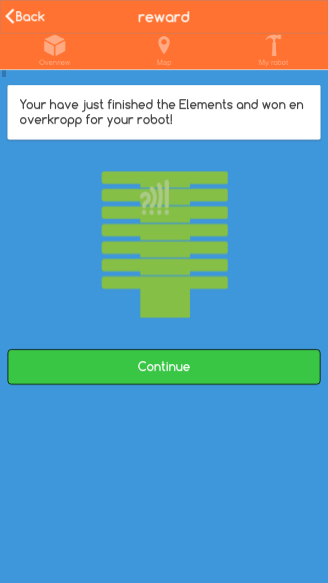
\includegraphics[width=0.5\textwidth]{images/app/reward.png}
    \caption{Example of part won when player wins a minigame.}
    \label{fig:reward}
\end{figure}
When all parts are collected one can submit the robot to Vitensenteret, where it can be seen on a screen with all submitted robots. This is done by pressing the green button at the top of the robot builder page when all parts are collected. One will be sent to a page where one can fill out the robot's name and your own, with a final preview of the robot. By clicking the Submit button at the bottom the robot will be submitted, and one will be taken to the robot overview. Fig. \ref{fig:finished} Fig. \ref{fig:robots_backend}
\begin{figure}[H]
    \centering
    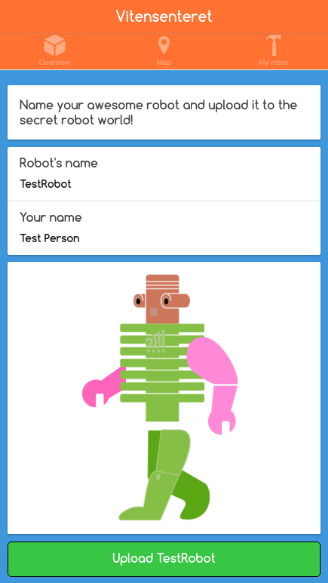
\includegraphics[width=0.5\textwidth]{images/app/finished.png}
    \caption{View of when a player has finished the game and is about to submit the Robot.}
    \label{fig:finished}
\end{figure}



\begin{figure}[H]
    \centering
    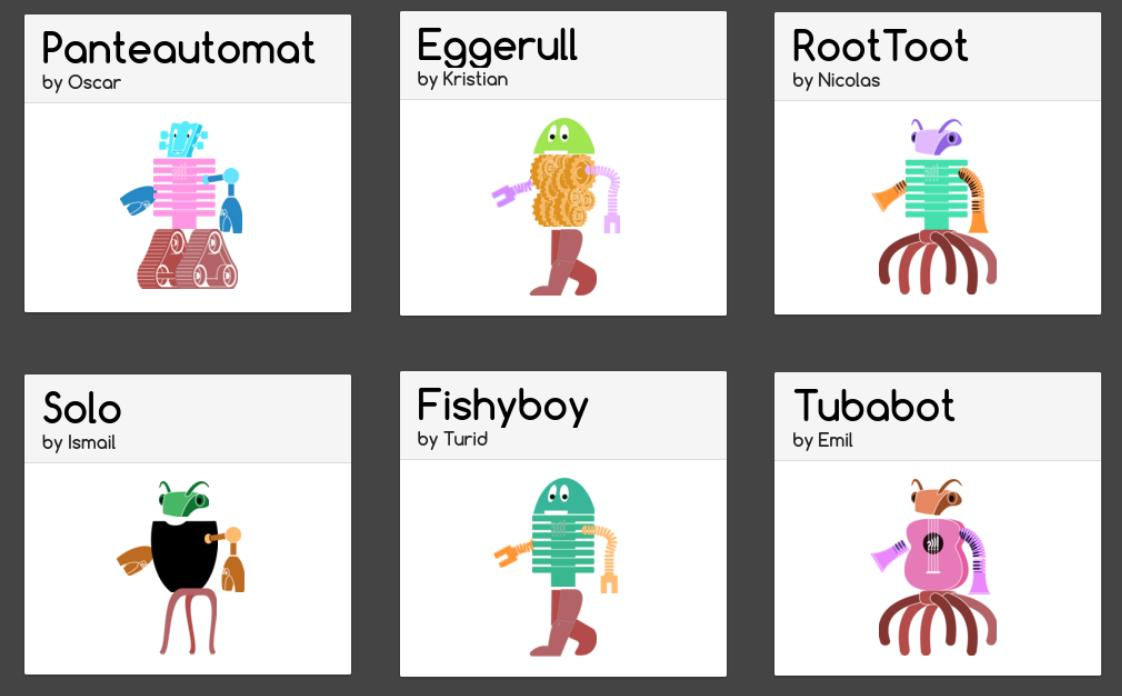
\includegraphics[width=0.5\textwidth]{images/app/robots_backend.jpg}
    \caption{The webpage with all the submitted robots.}
    \label{fig:robots_backend}
\end{figure}



\subsection{Quiz}
The quiz game uses questions found throughout the exhibition to quiz the player on different themes. Press the correct alternative to progress through the 11 questions. If one answers wrong the question will be asked again at the end. Game depicted in figure \ref{fig:Quiz}
\begin{figure}[H]
    \centering
    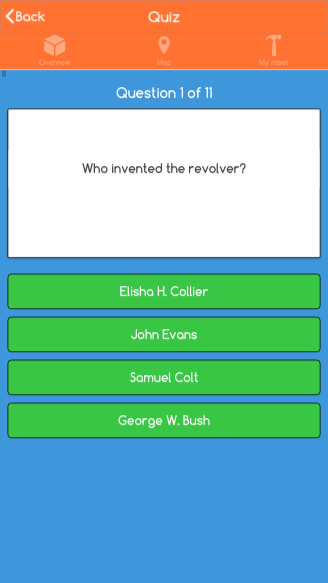
\includegraphics[width=0.5\textwidth]{images/app/Quiz.png}
    \caption{The ``Quiz" app view.}
    \label{fig:Quiz}
\end{figure}

\subsection{Elements}

\begin{figure}[H]
    \centering
    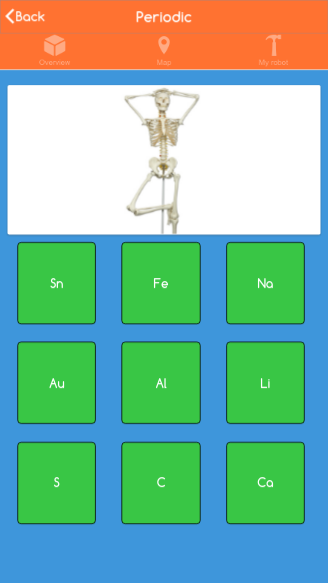
\includegraphics[width=0.5\textwidth]{images/app/Periodic.png}
    \caption{Periodic game}
    \label{fig:Periodic}
\end{figure}

The elements game (Grunnstoffer in norwegian) is a game where one is to find what chemical element the depicted item is made of, and is supposed to be played in front of the ``Table of elements" exhibit.
Search the exhibit for the displayed item, find what the scientific name of that element is, and press the corresponding button. A descriptive text of that element will then be shown, letting the player know if he was right or wrong. Game depicted in figure \ref{fig:Periodic}


\subsection{Color Lock}

\begin{figure}[H]
    \centering
    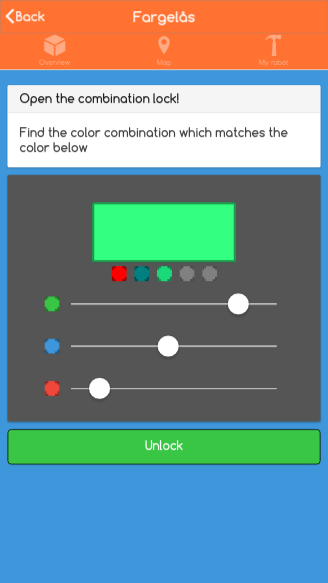
\includegraphics[width=0.5\textwidth]{images/app/colorlock.png}
    \caption{Color lock game}
    \label{fig:colorlock}
\end{figure}

The color lock game (Fargelås in norwegian) is a game where one is supposed to unlock a combination lock locked with different color combinations, and is linked to the color combination exhibit.\\\\
To play the game, drag the three sliders, each of which represents green, blue and red, so that they generate the same color that is displayed at the top. One is supposed to use the exhibit to find the combination, but a small preview of the current color combination can also be found under the large color rectangle. The ``Unlock" button will become active when the correct combination is entered, and will make the next color active. Game depicted in figure  \ref{fig:colorlock}.


\subsection{Melody Game}

\begin{figure}[H]
    \centering
    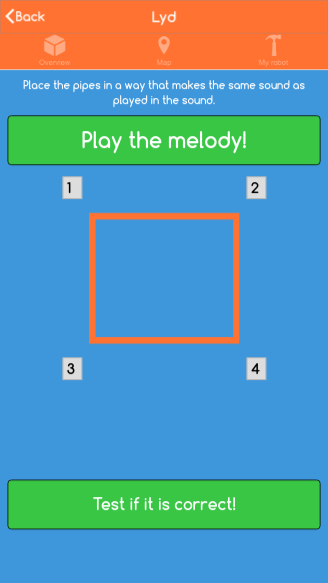
\includegraphics[width=0.5\textwidth]{images/app/Lyd.png}
    \caption{Melody game}
    \label{fig:Lyd}
\end{figure}

The melody game (melodispillet in norwegian) is a game where one is to rearrange metallic tubes in the rythm-exhibit to make the same sound as the app and input the position of the tubes into the app.\\\\
To play the game click ``Play the sound", listen to the sound, and re-create that sound with the tubes. You can then input the position of the tubes into the white dropdown boxes in the app and click the ``Test" button. The game is depicted in \ref{fig:Lyd}.


\subsection{Pipes}

\begin{figure}[H]
    \centering
    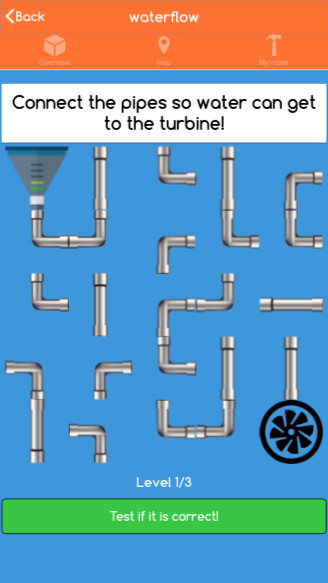
\includegraphics[width=0.5\textwidth]{images/app/waterflow.png}
    \caption{Waterflow game}
    \label{fig:waterflow}
\end{figure}

The Pipes game (Vannkobling in norwegian) is a game where one is to rotate the different pipes so that water can flow from the water container at the top left, to the turbine in the bottom right. This is done by simply pressing the pipe one wants to rotate until it is in the correct position. There are three levels, all of which have to be completed to win the game. The game can be played anywhere, but is supposed to be played in the water power room. The game is depicted in figure \ref{fig:waterflow}.


\subsection{Simon Says}

\begin{figure}[H]
    \centering
    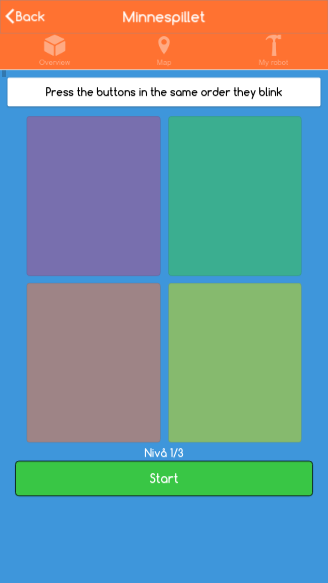
\includegraphics[width=0.5\textwidth]{images/app/Minnespillet.png}
    \caption{Simon says game}
    \label{fig:Minnespillet}
\end{figure}

The Simon Says game (Minnespillet in  norwegian) is a game where one has to remember in which order a series of blinking lights blink, to test the memory of the player. It can be played anywhere, is connected to the memory room.\\\\
To play it press the ``Start" button, watch the lights blink, and re-create the same sequence by pressing the correct colored squares. There are three levels, with increasing difficulty, all of which have to be completed to win the game. The game is depicted in figure \ref{fig:Minnespillet}.

\subsection{Shortest Path}

\begin{figure}[H]
    \centering
    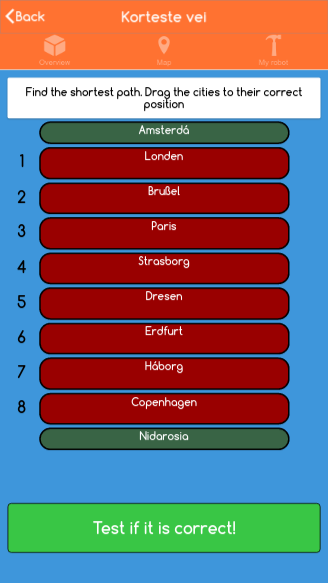
\includegraphics[width=\textwidth]{images/app/shortest.png}
    \caption{Shortesst path game}
    \label{fig:shortest}
\end{figure}

The Shortest Path game (Korteste veien in norwegian) is a game where one has to find the shortest signle path between multiple cities in Europe, where Amsterdam is the start and ``Nidarosia" or Trondheim is the end. A map and measuring tools can be found in the mathematics room, and must be used to measure the distances.\\\\

To play the game drag the red boxes into their correct positions and click the ``Check" button. If some of the cities are incorrectly placed they will remain red, but turn green when placed in the correct position. The game is depicted in Fig. \ref{fig:shortest}.


\section{Restarting your game}
To restart your game and delete all saved data go to the ``My Robot" tab, scroll to the bottom, press the red ``Delete my robot and restart" button and confirm the action. The application will then delete all saved data and reload the application.\\\\
This can be useful if one wants to replay the games, test out something, if there are any bugs, or if one has installed a new version of the app and some old data is stored.

\section{Troubleshooting}
\begin{itemize}
    \item If beacons don't work, try enabling Bluetooth on the phone, go into application settings and enable the Location permission for the app, and restart the game, as described in the ``Restarting your game" section above.
    \item If you chose the wrong language when the app started, restart the game as described in the ``Restarting your game" section above.
    \item If you can't install the app, try enabling ``Unknown sources" in settings.
\end{itemize}


\section{Known Issues}
\begin{itemize}
    \item Some views do not fit into a mobile screen, and the user has to scroll to see all elements.
    \item The application can not be installed on android phones with a version below 4.4 KitKat.
    \item On android 6.0.1 and above one has to manually allow location services to be used by the app (in the application settings) so that it can connect to Beacons.
\end{itemize}
